% Ellipse with its right focus at the origin: axes 2a,2b, focus offset ae,
% and semi-latus rectum p. Reference: handdraw/eccentric.png.
% Compile: pdflatex eccentric_tikz.tex
\documentclass[tikz,border=6pt]{standalone}
\usepackage{amsmath}
\usepackage{fix-cm}
\usetikzlibrary{arrows.meta}
\begin{document}
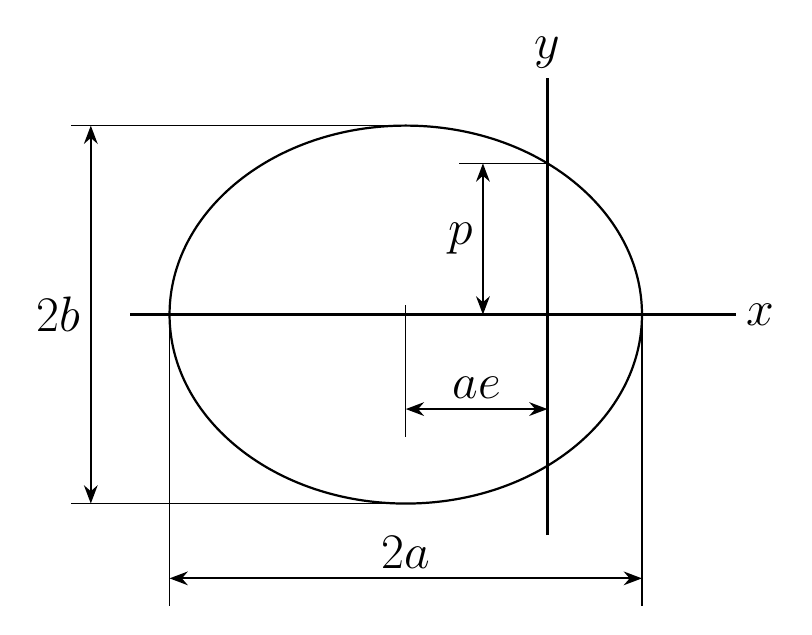
\begin{tikzpicture}[>=Stealth,thick,every node/.style={font=\fontsize{18}{22}\selectfont}]
  % a=3, b=2.4, c=ae=1.8, p=b^2/a=1.92.
  \draw (-1.8,0) ellipse [x radius=3,y radius=2.4];
  \draw (-5.3,0) -- (2.4,0) node[right] {$x$};
  \draw (0,-2.8) -- (0,3) node[above] {$y$};
  \draw[thin] (-6.05,2.4) -- (-1.8,2.4);
  \draw[thin] (-6.05,-2.4) -- (-1.8,-2.4);
  \draw[<->] (-5.8,-2.4) -- (-5.8,2.4) node[midway,left] {$2b$};
  \draw[thin] (-4.8,0) -- (-4.8,-3.7);
  \draw[thin] (1.2,0) -- (1.2,-3.7);
  \draw[<->] (-4.8,-3.35) -- (1.2,-3.35) node[midway,above] {$2a$};
  \draw[thin] (-1.8,.12) -- (-1.8,-1.55);
  \draw[<->] (-1.8,-1.2) -- (0,-1.2) node[midway,above] {$ae$};
  \draw[thin] (-1.12,1.92) -- (0,1.92);
  \draw[<->] (-.82,0) -- (-.82,1.92) node[midway,left] {$p$};
\end{tikzpicture}
\end{document}
